\documentclass[a4paper]{report}
\usepackage{a4wide}
\usepackage[utf8]{inputenc}
\usepackage{parskip}
\usepackage{hyperref}
\usepackage{epsfig}
\usepackage{background}
\usepackage{mathptmx}

% To avoid tikz error, see https://tex.stackexchange.com/questions/165929/semiverbatim-with-tikz-in-beamer
\makeatletter
\global\let\tikz@ensure@dollar@catcode=\relax
\makeatother

\backgroundsetup{
scale=1,
angle=0,
opacity=1,
contents={
\includegraphics[width=\paperwidth,height=\paperheight]{images/spi-front.jpg}}
}

\hypersetup{
  colorlinks   = true,
  urlcolor     = blue,
  linkcolor    = blue,
  pdfinfo = {
    Title = {SPI Annual Report 2021},
    Author = {Software in the Public Interest, Inc.},
    Keywords = {SPI, free software, open source, FOSS, annual report, charity, non-profit, 501c3},
  }
}

\begin{document}

\title{Software in the Public Interest, Inc.\\
2021 Annual Report}
\date{July XXX, 2022}

\maketitle

\newpage

\backgroundsetup{
scale=1,
angle=0,
opacity=1,
contents={
\includegraphics[width=\paperwidth,height=\paperheight]{images/spi-content.jpg}}
}

\hspace{1em}

To the membership, board and friends of Software in the Public Interest, Inc:

As mandated by Article 8 of the SPI Bylaws, I respectfully submit this annual report on the activities of Software in the Public Interest, Inc. and extend my thanks to all of those who contributed to the mission of SPI in the past year.

  \emph{-- Michael Schultheiss, SPI President}

\newpage

\tableofcontents

\newpage

\chapter{President's Welcome}
\label{sec:president}

  \emph{-- Michael Schultheiss, SPI President}

\chapter{Committee Reports}
\section{Membership Committee}

\subsection{Statistics}

On January 1, 2021 we had 232 contributing and 1173 non-contributing members.  On December 31, 2021 there were 243 contributing members and 1253 non-contributing members.  This is an increase of 11 contributing members and an increase of 80 non-contributing members.

\chapter{Board Report}
\section{Board Members}

Board members as of January 1, 2021:

\begin{itemize}
\item Michael Schultheiss (President)
\item Stephen Frost (Vice President)
\item Tim Potter (Secretary)
\item Martin Zobel-Helas (Treasurer)
\item Joe Conway
\item Luca Filipozzi
\item Forrest Fleming
\item Chris Lamb
\item Héctor Orón Martínez
\end{itemize}

Board members as of December 31, 2021:

\begin{itemize}
\item Michael Schultheiss (President)
\item Stephen Frost (Vice President)
\item Tim Potter (Secretary)
\item Héctor Orón Martínez (Treasurer)
\item Joe Conway
\item Forrest Fleming
\item Milan Kupcevic
\item Chris Lamb
\item Martin Zobel-Helas
\end{itemize}

\section{Board Changes}

Changes that occurred during the year:

\begin{itemize}

\item Luca Filipozzi resigned from the board in February 2021.  We'd like to thank Luca for his contributions!

\item The board appointed Milan Kupcevic as an interim director in April 2021.

\item On August 16, 2021 the board voted to appoint the following officers:

\begin{itemize}
\item President: Michael Schultheiss
\item Vice President: Stephen Frost
\item Secretary: Tim Potter
\end{itemize}

\item On September 13, 2021 the board voted to appoint the following officers:

\begin{itemize}
\item Treasurer: Héctor Orón Martínez
\end{itemize}

\end{itemize}

\section{Elections}

A board membership election was conducted in July 2021.  There were 3 board seats up for election.  Nominations were received from Stephen Frost, Milan Kupcevic, and Michael Schultheiss.  Since there were 3 nominations for 3 board seats, no vote was required and all three candidates were elected for a 3 year term.

\chapter{Treasurer's Report}

\chapter{Member Project Reports}

\section{New Associated Projects}

\subsection{Adélie Linux}

\href{https://www.adelielinux.org/}{Adélie} is an independent Linux distribution committed to integrity, privacy, and user freedom.  Adélie is lightweight and supports many 32- and 64-bit computer architectures. Adélie is designed for both desktop and server use.

\subsection{PMIx}

The \href{https://pmix.org/}{PMIx Standard Community Project} is governed by the PMIx Administrative Steering Committee (ASC). The ASC is a formal body that manages the PMIx Standard, PMIx Governance, and associated documents. The PMIx Standard document defines an API that provides libraries, tools, and resource managers with portable and well-defined access to commonly needed services in high-performance distributed and parallel computing systems.

\section{Projects No Longer Associated with SPI}

\begin{itemize}

\item OpenWrt joined Software Freedom Conservancy.

\item Performance Co-Pilot started using the OpenCollective Foundation platform to manage funds and no longer needs services from SPI.

\end{itemize}

\section{Updates from Associated Projects}

\subsection{0 A.D.}

\href{https://play0ad.com/}{0 A.D.} (pronounced ``zero ey-dee'') is a cross-platform, real-time strategy (RTS) game of ancient warfare. It is a historically-based war/economy game, in which the player must lead an ancient civilization, gather resources, and raise a military force to conquer enemy factions. 0 A.D. is open source software licensed under the GPL, and its art and sound assets are licensed under CC BY-SA. It is developed by Wildfire Games, a global community of game developers.

In 2021, we released two alpha versions, each with new features and improvements. For example, we made progress on improving pathfinding and reducing game lag, which improved the user experience immensely. We adjusted the gameplay balance, improved the graphics renderer and tweaked the in-game user interface. Additionally, we upgraded the game's JavaScript engine (SpiderMonkey), began using up-to-date compiler and code standards, and added a reinforcement learning component to the AI engine. As always, we added many new and amazing art assets as well.

Team members also presented the game at FOSS community events (such as FOSDEM) and on podcasts (such as Hanselminutes). Taken together, these outreach efforts helped raise awareness of 0 A.D. and facilitated recruitment of contributors.

We wish to extend our thanks to our generous donors and to SPI for helping us achieve this progress.

{\em Submitted by Aviv Sharon}

\subsection{Adélie Linux}

The \href{https://www.adelielinux.org/}{Adélie Linux} distribution underwent a \href{https://blog.adelielinux.org/2021/07/22/2021-state-of-the-adelie-linux-distribution/}{strategic change in leadership} to further refine and drive its mission.  \href{https://zv.io/about/}{Zach van Rijn}, former software engineer at IBM and computational modeler at Sanofi, succeeded A. Wilcox as the project's lead.

Adélie is a lightweight, \href{https://musl.libc.org/}{{musl-based}}, independent Linux platform for desktop and server use, committed to integrity, privacy, and user freedom.

In 2021, Adélie proudly \href{https://www.spi-inc.org/projects/adelielinux/}{accepted an invitation to join SPI}. We took major steps to improve community engagement, including redesigning our web site and services to make them easier to navigate and maintain.

We overhauled our core infrastructure after receiving several hardware donations. We moved into a co-location facility to accommodate short- and long-term projects as we expand into scientific computing and research collaborations.

\href{https://actionretro.com/}{Action Retro} published a \href{https://www.youtube.com/watch?v=AArGaJGFVH4}{surprise feature} showing that Adélie is also a viable desktop distribution for '90s era 32-bit PowerPC Macintosh hardware.

We attended \href{https://alpinelinux.org/conf/}{{AlpineConf 2021}}, the inaugural Alpine Linux conference, to discuss matters relevant to the musl ecosystem. Behind the scenes, we're working closely with these projects to improve the state of free and open source software.

We \href{https://blog.adelielinux.org/2021/12/31/new-year-new-builders/}{wrapped up 2021}, despite beginning the year without access to any build servers (long story), by building and testing packages for all six of our supported architectures: ARM, POWER, and x86 in both 32- and 64-bit address models.

For 2022, you can look forward to our third release candidate, RC3, and hopefully our 1.0 general release. Please follow \href{https://blog.adelielinux.org/}{our blog} and \href{https://www.adelielinux.org/contact/}{social media accounts} to stay informed about our progress!

{\em Submitted by Zach van Rijn}

\subsection{Arch Linux}

\href{https://archlinux.org/}{Arch Linux} is a lightweight and flexible Linux distribution that tries to \textit{Keep It Simple}.  This year we continued to work on usability and community outreach with a focus on technical improvements.

A man pages indexing site at man.archlinux.org launched in January, which publishes the man pages of all our packages and allows searching and browsing.

As of April, our installation medium provides a guided installer called \texttt{archinstall} as an addition to the default method based on the installation guide. The guided installer offers various customization features including a plugin and profile system aimed at making the installation process more convenient.

In May we moved all our official IRC channels from Freenode to Libera.

In the second half of the year our arch-repo-management project gained features to provide daily validation checks of package repository databases.  The project’s tooling is meant to replace the aging db scripts in the future, which is used for package repository management.

{\em Submitted by Levente Polyák}

\subsection{FFmpeg}

\href{https://www.ffmpeg.org/}{FFmpeg} is a complete, cross-platform solution to record, convert and stream audio and video. It is used as the foundation platform of many projects dealing with multimedia, both open source and proprietary, and is used extensively by several web-based multimedia conversion and processing services.

In the year 2021 FFmpeg delivered the \href{https://git.ffmpeg.org/gitweb/ffmpeg.git/blob/refs/heads/release/4.4:/RELEASE_NOTES}{4.4 formal release} and many security updates of old releases. A complete list of changes can be found in \href{https://git.ffmpeg.org/gitweb/ffmpeg.git/blob/HEAD:/Changelog}{the changelog}.

FFmpeg joined the GSoC 2021 program, with a total of \href{https://trac.ffmpeg.org/wiki/SponsoringPrograms/GSoC/2021/Results}{two completed projects}.

Due to the pandemic crisis, no meetings and conferences were attended by FFmpeg developers during the year.

{\em Submitted by Stefano Sabatini}

\subsection{Haskell.org}

\href{https://www.haskell.org/}{Haskell.org} is an infrastructure hub for the Haskell programming language community. In 2021, it helped launch the Haskell Foundation, an organization which has raised over \$500,000 to support improvement of the Haskell ecosystem. It also continued its many ongoing community support initiatives, including running Google Summer of Code for Haskell and maintaining the haskell.org website.

{\em Submitted by Ryan Trinkle}

\subsection{LibreOffice}

In 2021, The Document Foundation (TDF) released two major versions of \href{https://www.libreoffice.org/}{LibreOffice}, starting with LibreOffice 7.1 in February. A new dialog was added which lets users select their desired user interface design on first startup (including the regular menu+toolbar setup, and NotebookBar alternative). In Writer, a new Style Inspector was created to display the attributes of Paragraph and Character Styles, and manually formatted (Direct Formatting) properties. In Calc, significant speed improvements for Autofilter and find/replace operations were implemented, while the possibility to add visible signatures to existing PDF files in Draw was included too. On top of the new features, there were many other general improvements to performance, compatibility and stability.

Later in the year, on August 19, TDF released LibreOffice 7.2. Based on the LibreOffice Technology platform for personal productivity on desktop, mobile and cloud, it provided a large number of interoperability improvements with Microsoft's proprietary file formats. In addition, LibreOffice 7.2 Community offered numerous performance improvements in handling large files, opening certain DOCX and XLSX files, managing font caching, and opening presentations and drawings that contain large images. There were also drawing speed improvements when using the Skia back-end that was introduced with LibreOffice 7.1.

{\em Submitted by Mike Saunders}

\subsection{ns-3}

\href{https://www.nsnam.org}{ns-3} is a discrete-event, packet-level network simulator with an emphasis on networking research and education.

In 2021, ns-3 made three regular software releases of the main simulator, and published an additional release of its Direct Code Execution environment framework.  Among the most significant or extensive changes were the addition of models of the current Wi-Fi 6 standard, new congestion control models for TCP, and improvements to the antenna and channel models for 4G LTE simulations.

ns-3 also mentored three student projects in the 2021 edition of Google Summer of Code, and organized its thirteenth annual academic workshop, featuring twelve technical paper presentations and numerous lightning talks and tutorial sessions.  The workshop was held online due to the pandemic.

{\em Submitted by Tom Henderson}

\subsection{OFTC}

\href{https://oftc.net/}{OFTC} aims to provide stable and effective collaboration services to members of the community in any part of the world.

We're excited to be working towards updating our software stack while still continuing to support communities that use our services.

{\em Submitted by Tom Wesley}

\subsection{Open Bioinformatics Foundation}

The \href{https://www.open-bio.org/}{Open Bioinformatics Foundation} (OBF) is a non-profit, volunteer-run group that promotes open source and open science in biological research. At the public Board meeting in September 2021, two new Board members were elected: Hilyatuz Zahroh (Genetics Research Centre, Universitas YARSI, Indonesia) and Caleb Kibet (International Center of Insect Physiology and Ecology, Kenya).

The OBF adopted a Code of Conduct in January 2022 after being approved by a membership-wide referendum. OBF participated in Google Summer of Code 2021 and has been accepted for 2022.  OBF Event Fellowships were awarded to 21 people in the past year to attend relevant virtual events. We sponsored two ISCBacademy talks: Mad Price Ball (Open Humans Foundation), ``Open Sourcing Ourselves -- Together'' (September 2021); and Yo Yehudi (Open Life Science), ``Growing open source communities with internships'' (February 2022).

OBF's most important event is the annual Bioinformatics Open Source Conference (BOSC). BOSC 2021 was held online July 29-30, 2021, as part of ISMB/ECCB 2021. One of the keynote speakers (Thomas Hervé Mboa Nkoudou, a leader in the biotech maker movement in Africa) delivered his keynote talk in French with English subtitles---a first for ISMB. In 2021, BOSC began offering honoraria to keynote speakers, in recognition of the fact that not all researchers are privileged to be able to gift their time. 20 BOSC 2021 participants from around the world were offered free registration for the virtual meeting. BOSC 2022 will take place July 13-14, 2022, as part of ISMB 2022 in Madison, Wisconsin, USA (with an online participation option).

{\em Submitted by Nomi Harris}

\subsection{OpenEmbedded}

\href{https://www.openembedded.org/}{OpenEmbedded} is a build system that creates custom Linux distributions for devices running Linux. Traditionally used for creating images for embedded devices, OpenEmbedded is now used all over to create small images for Internet of things (IoT) devices, to large images pushing into the desktop space.  Over the past year, we see additional users who build edge routers for IoT applications and images to deploy in popular containers systems.

To support the OpenEmbedded developer community, we work with the Yocto Project to arrange developer meetings twice a year. This year was challenging with the pandemic ending in person meetings. We did assist the Yocto Project with a couple of virtual events and hosted a virtual developer meeting.

{\em Submitted by Philip Balister}

\subsection{Open MPI}

The \href{https://www.open-mpi.org/}{Open MPI} community is a collection of academics, researchers, and vendors who continue to develop cutting-edge technology for today's most-demanding High Performance Computing (HPC) environments.

The community continues to maintain stable release series (v4.0.x and v4.1.x), even while working towards an aggressive new release series (v5.1.x).

In 2021:

\begin{itemize}

\item The community released v4.0.6 and v4.0.7.  v4.0.7 is expected to be the end of the v4.0.x series.

\item The community also released v4.1.1 and v4.1.2.  More releases are expected on this stable release series.

\item As with 2020, a major area of focus is the upcoming v5.0.x series. This series includes major under-the-covers changes to Open MPI's architecture and infrastructure, as well as several new features from the MPI-4.0 standard (which was ratified on June 9, 2021).  The v5.0.x series has taken longer than expected; we hope to release it in 2022.

\end{itemize}

The Hardware Locality (\texttt{hwloc}) sub-project had a bug-fix release (v2.4.1) and several minor releases: v2.5.0, v2.6.0, and v2.7.0.  Continuing prior release norms, the minor releases mainly deal with updates for new hardware and vendor form factors in advanced computing platforms.

{\em Submitted by Jeff Squyres}

\subsection{OpenSAF}

\href{https://opensaf.sourceforge.io/}{OpenSAF} is a high availability middleware, which helps in achieving 99.999\% of service availability to business and mission critical applications. It is the fastest and the most efficient middleware implementation of AIS specifications from SA Forum. OpenSAF is being used mostly in telecom and defence applications worldwide. OpenSAF can detect fault and perform recovery in few milliseconds.

In 2021, we made significant contributions to OpenSAF. We delivered 3 major releases:

\begin{itemize}

\item \href{https://sourceforge.net/p/opensaf/wiki/NEWS-5.21.03/}{OpenSAF-5.21.03}

\item \href{https://sourceforge.net/p/opensaf/wiki/NEWS-5.21.06/}{OpenSAF-5.21.06}

\item \href{https://sourceforge.net/p/opensaf/wiki/NEWS-5.21.09/}{OpenSAF-5.21.09}

\end{itemize}

We contributed 10 enhancements in all of these releases.

{\em Submitted by Nagendra Kumar}

\subsection{OpenZFS}

\href{https://openzfs.org/}{OpenZFS} held its annual Developer Summit online in November, 2021. The successful event had 9 presentation from people at 5 companies and one independent member of the community. There were approximately 400 attendees over the course of the summit and ~100 people who attended the full day.  Several of the presentation videos have received over 1000 views since the summit.

The main technical work was DRAID in OpenZFS 2.1. DRAID is a new distributed variant of RAIDZ which enables dramatically faster resilver times using integrated hot spares. Full redundancy can be restored to the pool in a fraction of the time normally required to do a full disk replacement.

{\em Submitted by Matthew Ahrens}

\subsection{PMIx}

The \href{https://pmix.github.io/}{PMIx Standardization community} is an international group spanning academia, research institutions, and industry vendors. Our collective focus is on refining and extending the PMIx interface to support existing and future parallel and distributed workloads in their needs to connect with various system services in cloud, data center, and HPC environments.

The community released the PMIx Standard v4.1 document in October 2021. This document includes clarifications and a new chapter on storage hierarchy inspection. In 2021 the community worked hard on clarifying semantics and interfaces in the PMIx standard.  Additionally, the PMIx community added a new set of use cases to the forthcoming v5.0 release. These use cases provide an entry point to new users of the PMIx standard.

{\em Submitted by Josh Hursey and Kathryn Mohror}

\subsection{PostgreSQL}

In 2021 \href{https://www.postgresql.org/}{PostgreSQL} was once again able to release a new major version, PostgreSQL 14. We are especially happy with this release and think it will become a critical version for users moving forward. In particular, this release builds on the past few releases to improve index management and performance, and also includes improvements to the autovacuum process to more aggressively handle transaction wrap-around scenarios, which we think considerably improve the overall experience working with PostgreSQL.

As for the PostgreSQL community, we continued with several initiatives including our participation in Google Summer of Code and our contributor appreciation program. We also saw our community start to take our first steps back towards in-person events, with mostly localized meetups and a few regional conferences, but with an eye towards an increasing number of events to come in 2022.

{\em Submitted by Robert Treat}

\subsection{Privoxy}

In 2021, three \href{https://www.privoxy.org/}{Privoxy} releases were announced.

For the first time in Privoxy's history work was done that is going to be paid with project funds held by SPI.

The first funded project was leveraging curl's tests suite to test Privoxy, the second project was using WolfSSL as TLS backend for HTTPS inspection.

Both projects are currently in the review state and are expected to be part of a Privoxy release in 2022.

{\em Submitted by Fabian Keil}

\subsection{Translatewiki.net}

\href{https://translatewiki.net/}{Translatewiki.net} is an online translation platform for free and open source projects and volunteer translators. This year we saw a modest growth in activity. 1,046 new translators signed up to be part of our community and 1,627 active translators made over half a million translation updates during the year. Additionally, 57 new software projects or their components were added for translation.

On the development side, we improved translation updates in many ways. We implemented removal of translations in languages falling under a certain completion threshold, fully automated translation updates with strong synchronization guarantees to avoid overriding or corrupting any translations, and fully automated translation backports to supported release branches of MediaWiki on a weekly schedule.

{\em Submitted by Niklas Laxström}

\subsection{Tux4Kids}

2021 saw two releases of \href{https://tuxpaint.org/}{Tux Paint}, in June and November.

Between the two versions, we added the following new features:

\begin{itemize}

\item Gradient and freehand variations added to the bucket Fill tool

\item Support for angled brushes in the Paint and Line tools

\item Nine new ``Magic'' effect tools were added, and updates to some others

\item The Magic tools were split into groups

\item An option was added to scale the user interface; useful for high-DPI monitors, small mobile devices, and users utilizing eye-gaze trackers)

\item User documentation was reorganized and overhauled, and now allows for easier and more consistent translation

\item The ``Tux Paint Config'' settings tool (for parents/teachers) had its UI cleaned up and also supports larger and higher-DPI displays

\item A new gallery was added to the Tux Paint website, showcasing some of the most incredible work done by children and adults around the world

\end{itemize}

This was on the heels of two releases in mid- and late-2020, with many more updates already under way in 2022.

{\em Submitted by Bill Kendrick}

\subsection{X.Org}

The \href{https://www.x.org/}{X.Org} and \href{https://www.freedesktop.org}{freedesktop.org} communities help to create a free and open accelerated graphics stack, including major components such as the DRM kernel graphics subsystem, Mesa 3D graphics library, Wayland compositors and the X Window System.

In 2021, we've been supporting the community through various services we provide such as the gitlab.freedesktop.org hosting infrastructure. We're also working on trying to start up discussions with the MIPI alliance to make it easier for open source projects to implement various MIPI related specifications.

And for the X.org Developer's Conference in 2021, we managed to secure 11 sponsors!

{\em Submitted by Lyude Paul}


\appendix
\chapter{About SPI}

SPI is a non-profit organization which was founded to help organizations develop and distribute open hardware and software. We encourage programmers to use the GNU General Public License or other licenses that allow free redistribution and use of software, and hardware developers to distribute documentation that will allow device drivers to be written for their product.

SPI was incorporated as a non-profit organization on June 16, 1997 in the state of New York. Since then, it has become an umbrella organization for projects from the community.

In 1999, the Internal Revenue Service (IRS) of the United States government determined that under section 501(a) of the Internal Revenue Code SPI qualifies for 501(c)(3) (non-profit organization) status under section 509(a)(1) and 170(b)(1)(A)(vi). This means that donations made to SPI and its supported projects are tax-deductible as charitable donations for US taxpayers.

\newpage

\pagestyle{empty}

\backgroundsetup{
scale=1,
angle=0,
opacity=1,
contents={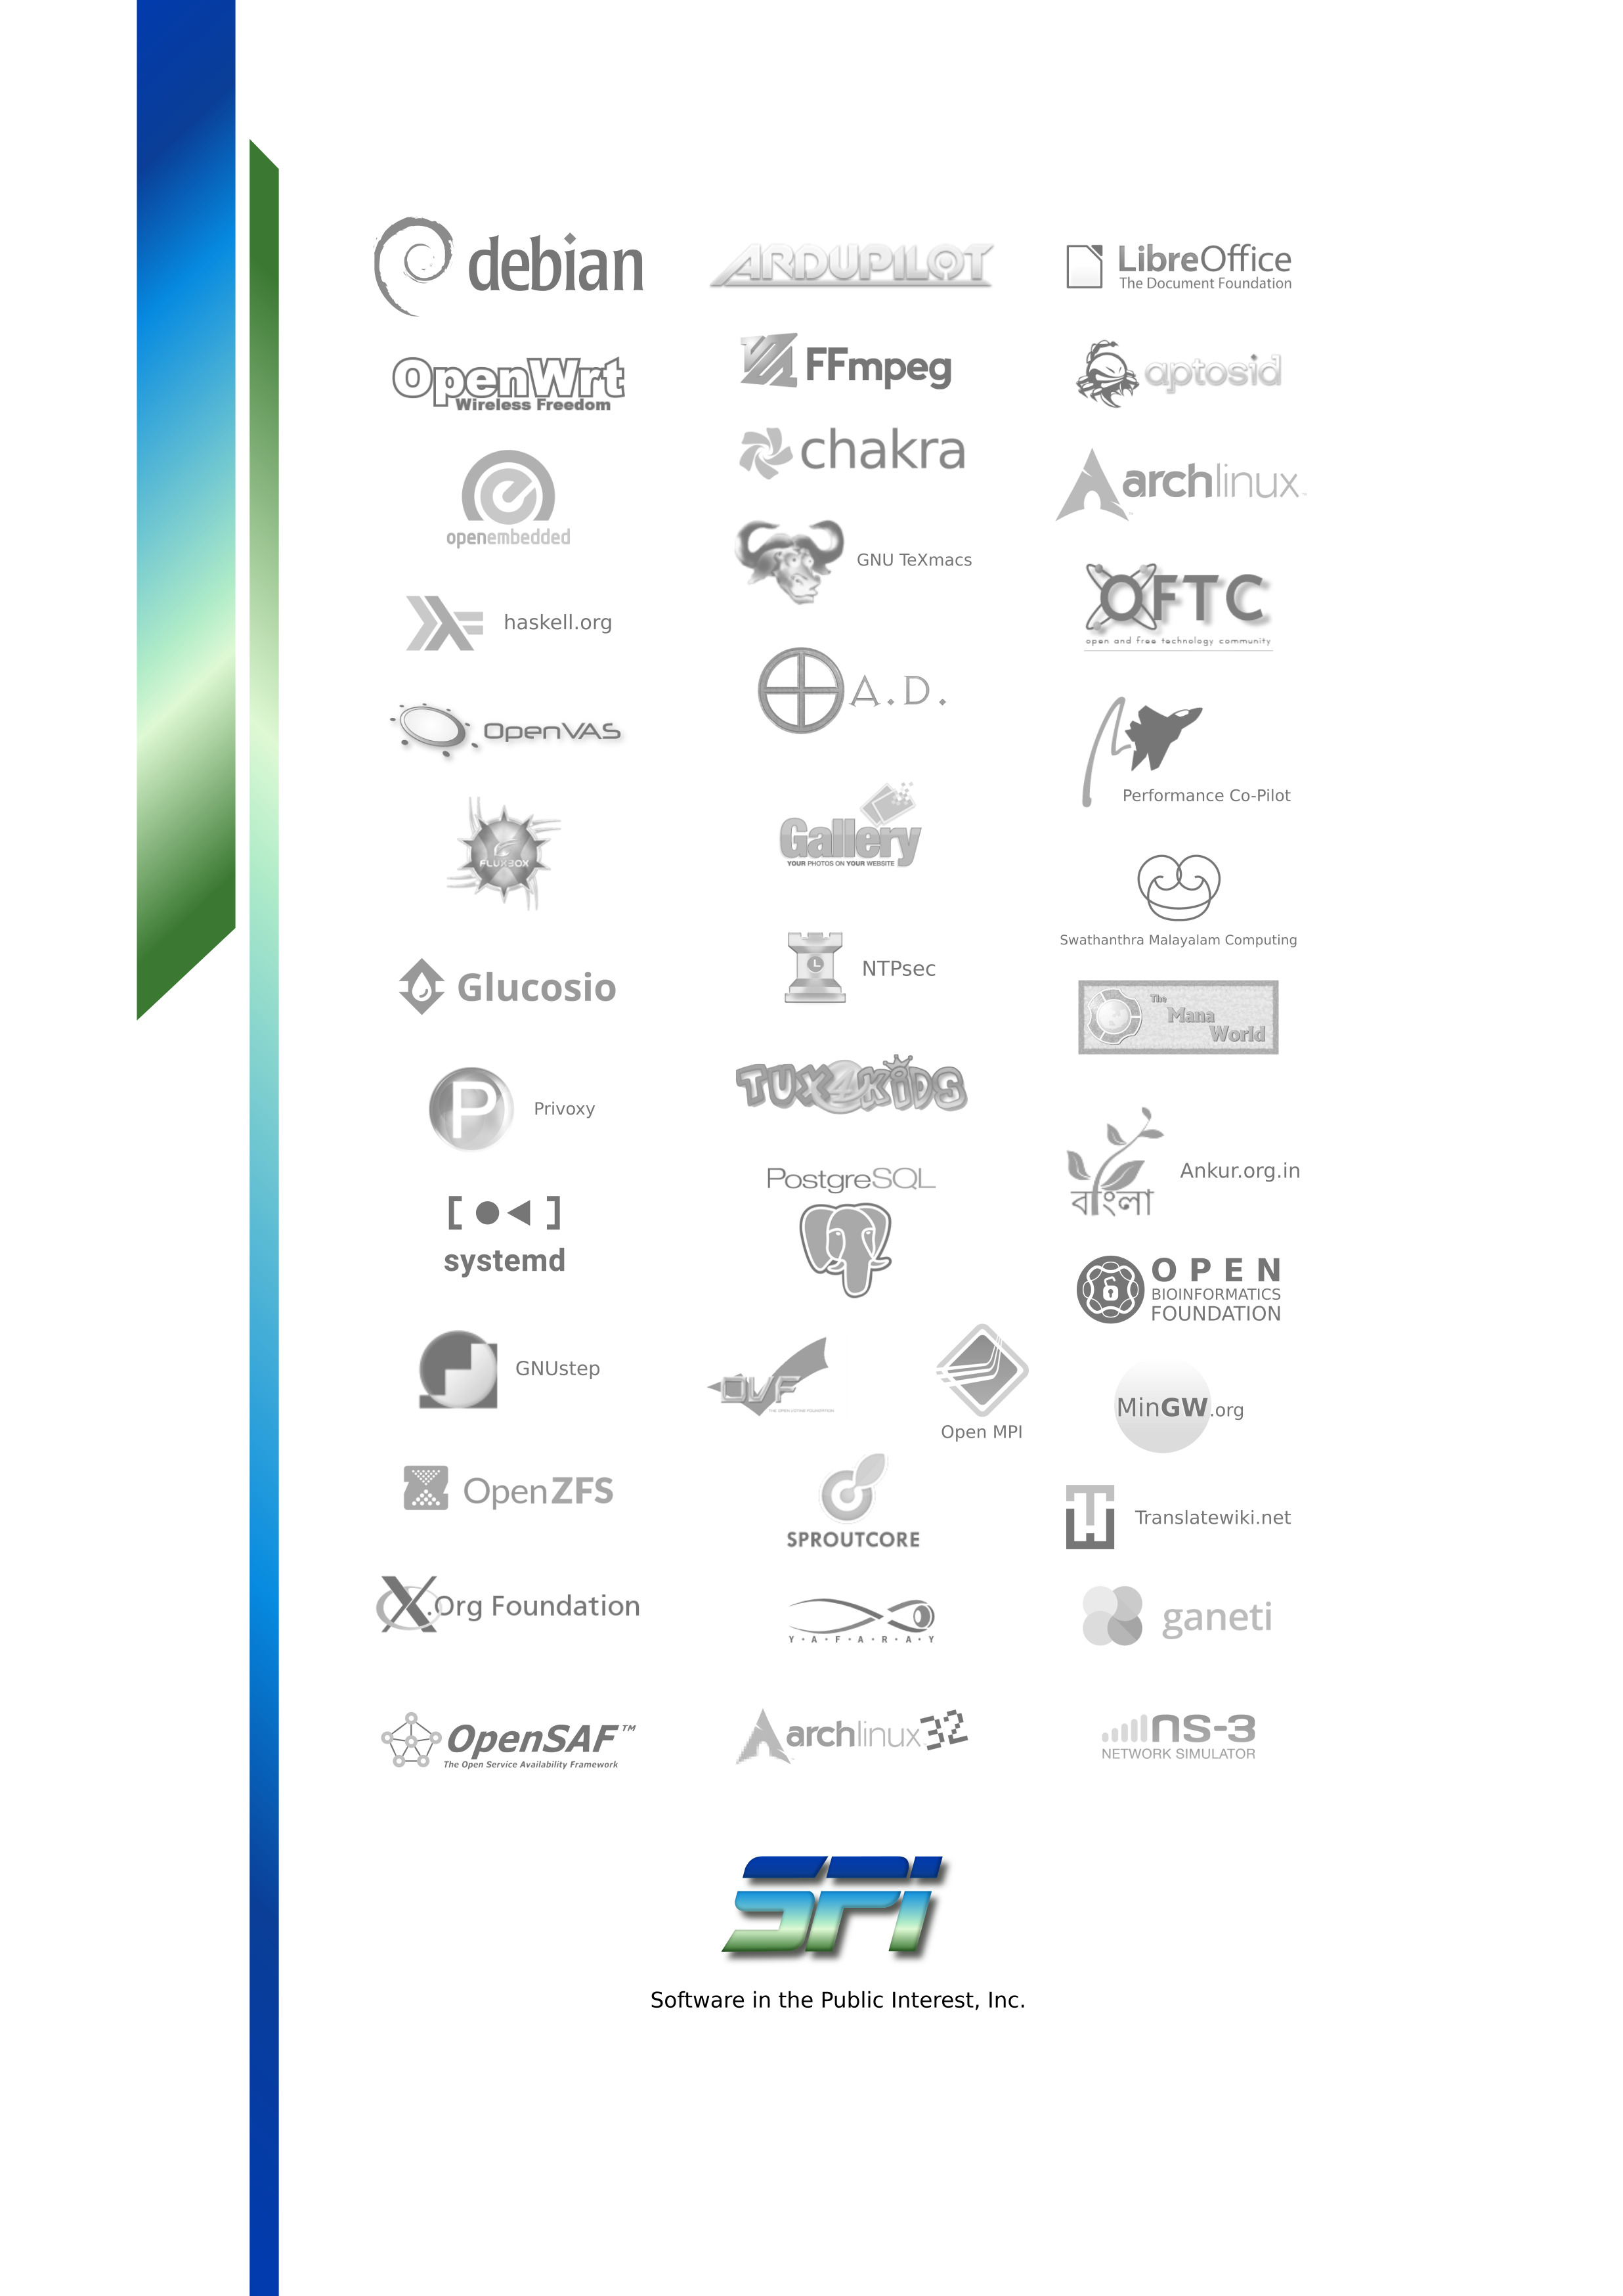
\includegraphics[width=\paperwidth,height=\paperheight]{images/spi-back-2020.jpg}}
}

\null

\end{document}
% Keep this at the bottom, thanks.
% Local Variables:
% TeX-master: "report"
% End:
